\section{Attention-based Decoding Sequences}
\begin{frame}{Decoding Sequences with Attention}
  \textbf{Attention-Based Decoding -- Overview}
  \begin{itemize}
    \item[$\blacktriangleright$]
      The decoder uses attention to select relevant encoder hidden states at each decoding step.
  \end{itemize}
  \textbf{Combines:}
  \begin{itemize}
    \item[] $\bullet$ Previous decoder state
    \item[] $\bullet$ Encoder hidden states
    \item[] $\bullet$ Attention context vector
  \end{itemize}
  \begin{itemize}
    \item[$\blacktriangleright$]
      The output at time $t$:
      \begin{equation*}
        y_t = \mathrm{Decoder}(y_{t-1}, \text{context}_t)
      \end{equation*}
  \end{itemize}
\end{frame}

\begin{frame}{Attention-Based Decoding}
  \centering
  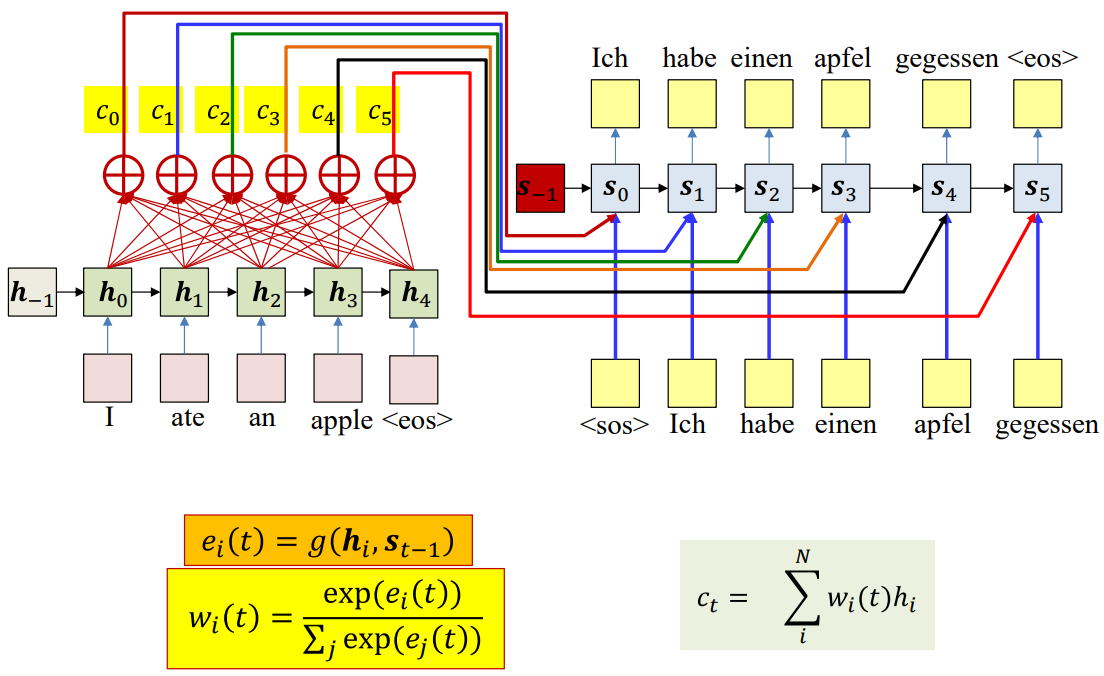
\includegraphics[width=0.7\paperwidth,height=0.49\paperheight,keepaspectratio]{images/attention-deep-dive/attention_rnn_context_per_step.png}

  {\scriptsize Source: after CMU 11-785 (Spring 2024), Lecture 18: Sequence to Sequence Models \& Attention, slides~28 and~31.}

  \begin{itemize}
    \item[$\blacktriangleright$] Every encoder state $h_i$ is scored against the previous decoder state, $e_i(t) = g(h_i, s_{t-1})$, and the scores are softmaxed into weights $w_i(t)$.
    \item[$\blacktriangleright$] Those weights already form a distribution, so the context is the plain weighted sum $c_t = \sum_i w_i(t)\, h_i$.
  \end{itemize}
\end{frame}

\begin{frame}{Decoding - Steps}
  \begin{enumerate}
    \item \textbf{Compute query}: Generate a query vector from the current decoder hidden state.
    \item \textbf{Align with encoder outputs}: Compare the query with encoder outputs (keys) to measure relevance.
    \item \textbf{Get attention weights}: Apply softmax to the alignment scores to obtain attention weights.
    \item \textbf{Compute context}: Calculate the context vector as the weighted sum of encoder outputs using the attention weights.
    \item \textbf{Feed into decoder}: Use the context vector and previous outputs as input for the next decoding step.
  \end{enumerate}
\end{frame}

\begin{frame}{Attention}
  \centering
  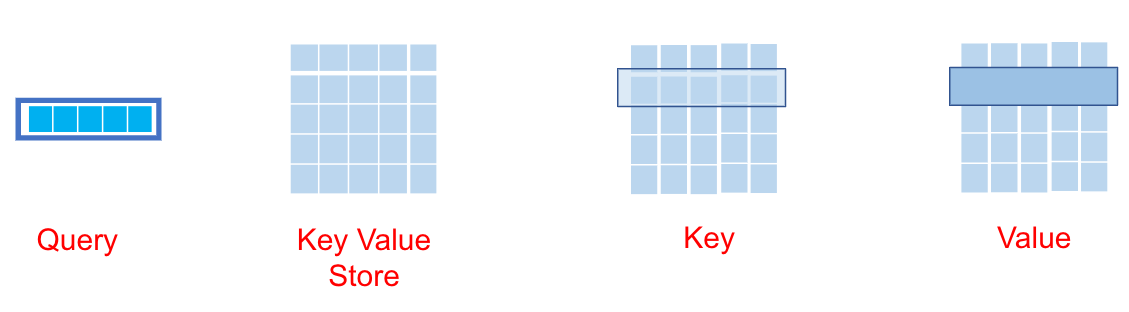
\includegraphics[width=0.7\paperwidth,height=0.66\paperheight,keepaspectratio]{images/attention-deep-dive/attention_qkv_matrix_query_key_value.png}

  {\scriptsize Source: CMU 11-785 (Spring 2024), Lecture 19: Transformers and Newer Architectures, slide~42.}
\end{frame}

\begin{frame}{Attention}
  \centering
  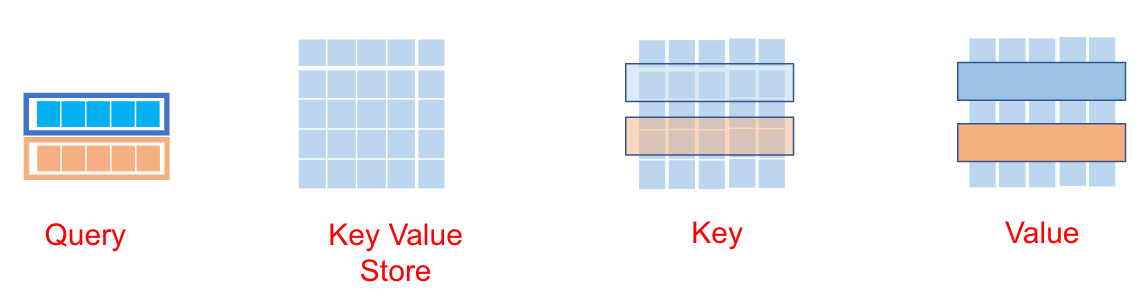
\includegraphics[width=0.7\paperwidth,height=0.66\paperheight,keepaspectratio]{images/attention-deep-dive/attention_qkv_two_query_rows.png}

  {\scriptsize Source: CMU 11-785 (Spring 2024), Lecture 19: Transformers and Newer Architectures, slide~43.}
\end{frame}

\begin{frame}{Attention}
  \centering
  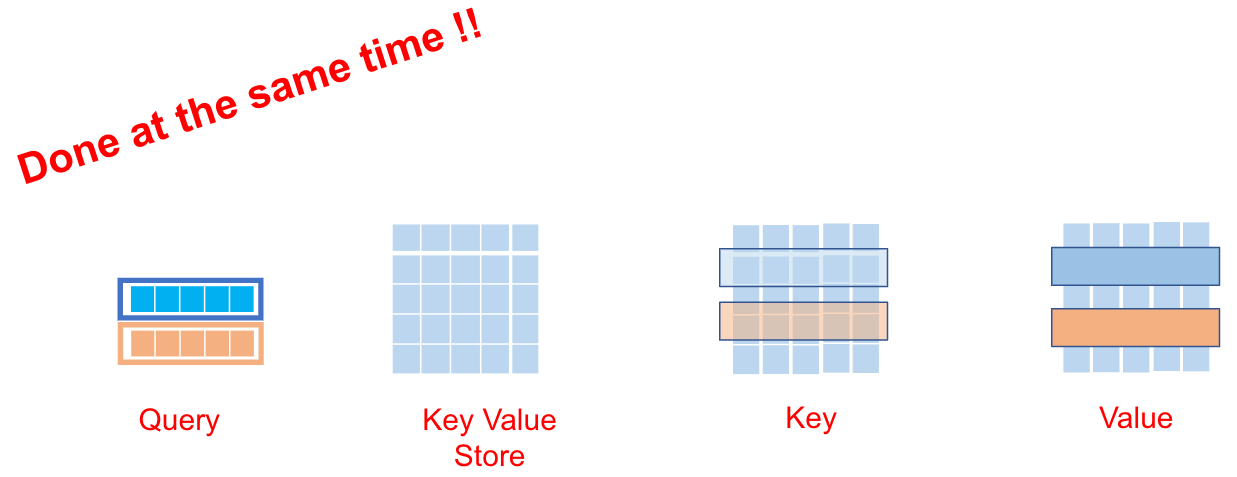
\includegraphics[width=0.7\paperwidth,height=0.66\paperheight,keepaspectratio]{images/attention-deep-dive/attention_qkv_parallel_same_time.png}

  {\scriptsize Source: CMU 11-785 (Spring 2024), Lecture 19: Transformers and Newer Architectures, slide~44.}
\end{frame}

\begin{frame}{Attention}
  \centering
  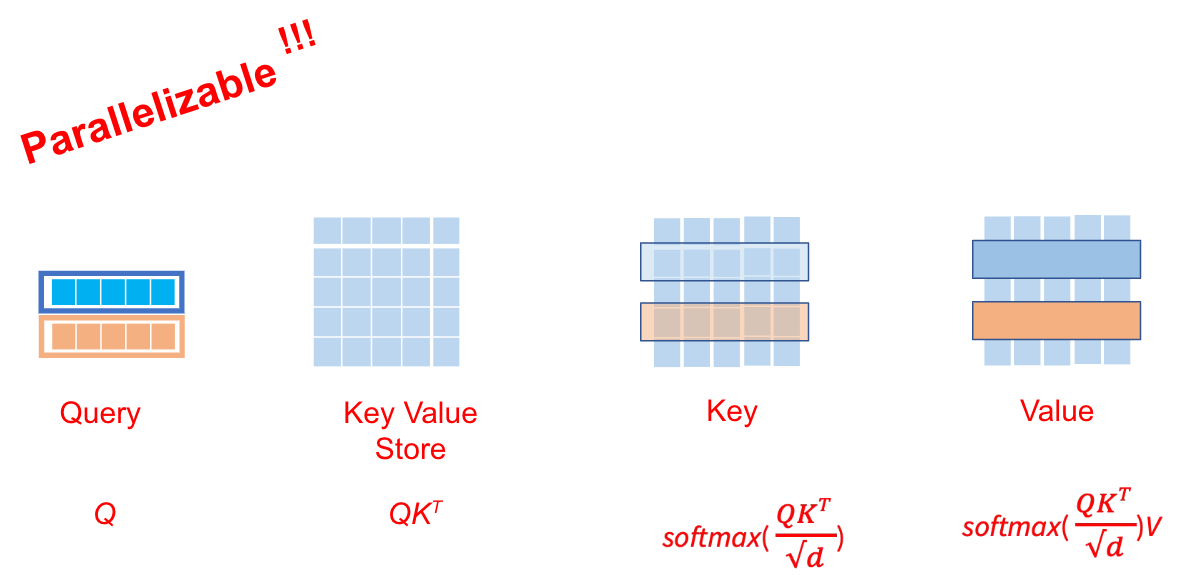
\includegraphics[width=0.7\paperwidth,height=0.66\paperheight,keepaspectratio]{images/attention-deep-dive/attention_qkv_parallel_formula.png}

  {\scriptsize Source: CMU 11-785 (Spring 2024), Lecture 19: Transformers and Newer Architectures, slide~45.}
\end{frame}

\begin{frame}{Self-Attention and Cross-Attention}
  The same scoring machinery serves two arrangements, distinguished only by where $\mathbf{Q}$, $\mathbf{K}$ and $\mathbf{V}$ are projected from.
  \begin{itemize}
    \item[$\blacktriangleright$] \textbf{Cross-attention:} the query comes from the decoder state and the keys and values from the encoder states, so the decoder reads the source sentence. This is the arrangement used so far.
    \item[$\blacktriangleright$] \textbf{Self-attention:} query, key and value are all projected from one and the same sequence, so every token is re-expressed as a weighted sum of its neighbours.
  \end{itemize}
  \vspace{0.5em}
  The next slides trace self-attention over the input ``I ate an apple \textless eos\textgreater'', one score at a time. No token's output depends on another token's output, so every position can be computed at once: this is what makes the mechanism parallelizable.
\end{frame}

\begin{frame}{Attention}
  \centering
  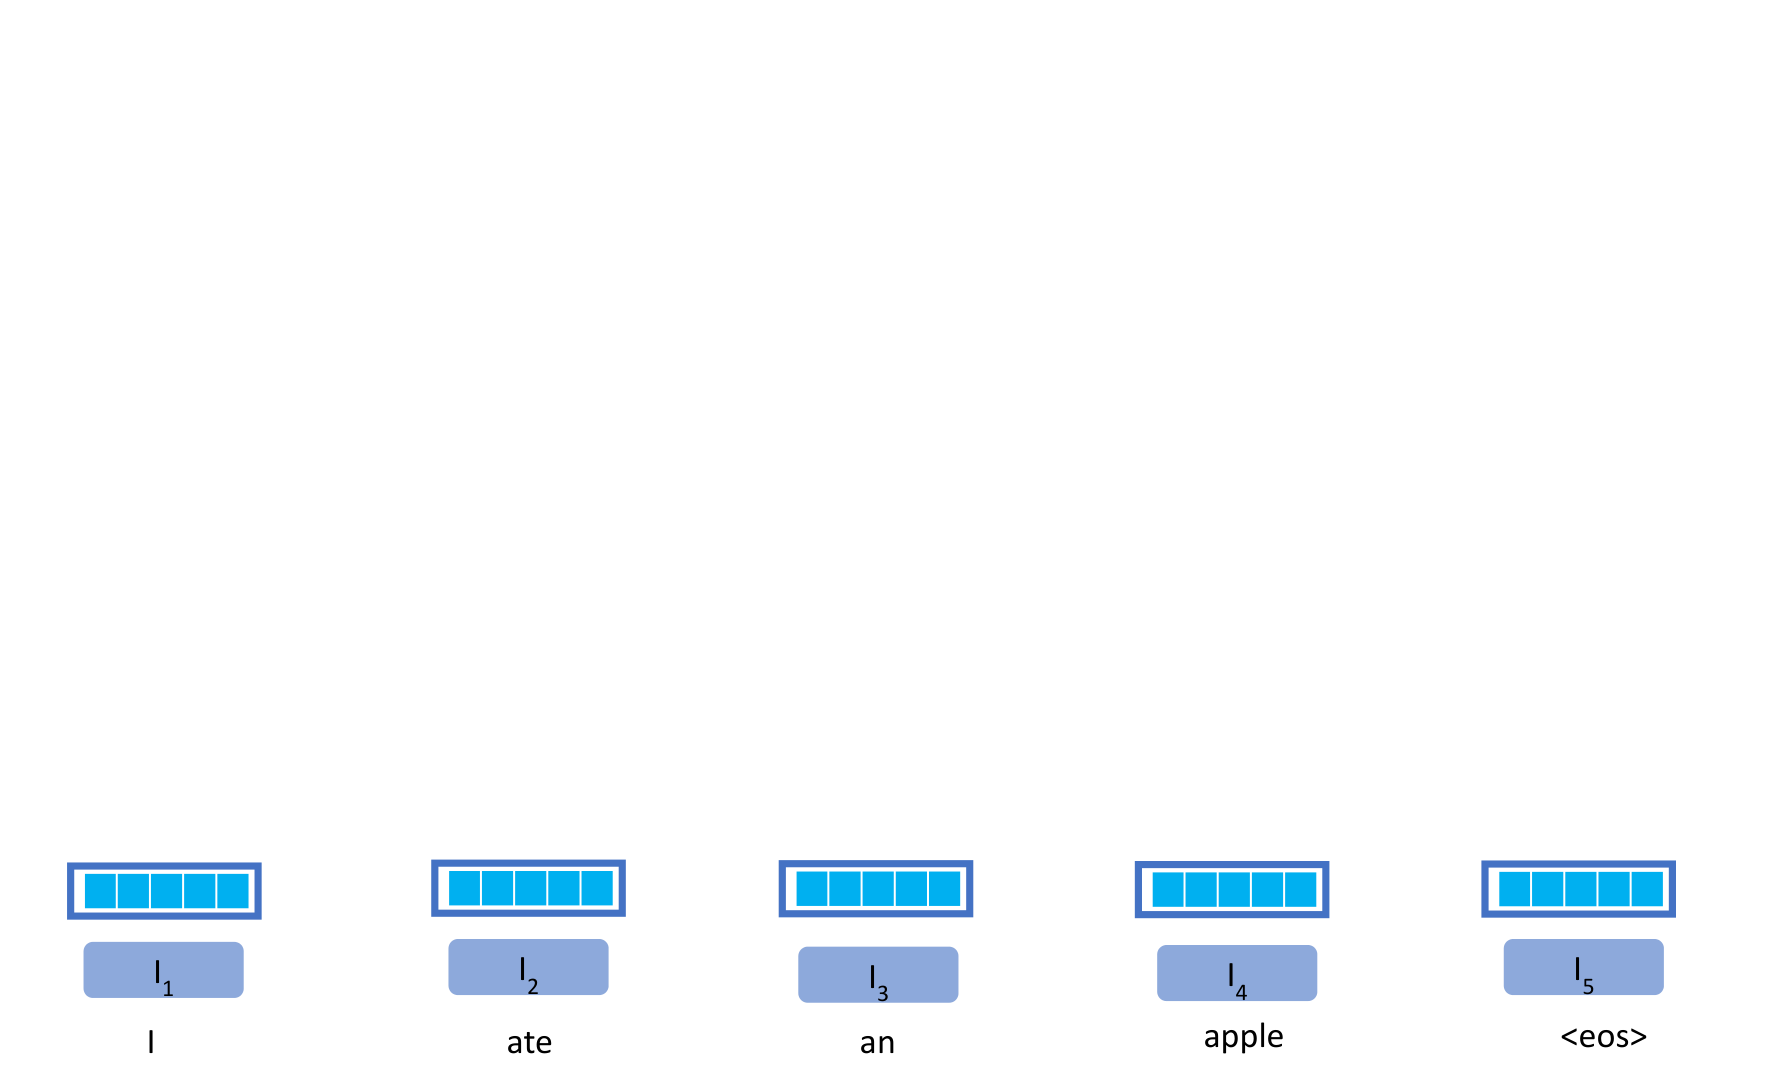
\includegraphics[width=0.7\paperwidth,height=0.66\paperheight,keepaspectratio]{images/attention-deep-dive/attention_input_embeddings_tokens.png}

  {\scriptsize Source: CMU 11-785 (Spring 2024), Lecture 19: Transformers and Newer Architectures, slide~46.}
\end{frame}

\begin{frame}{Attention}
  \centering
  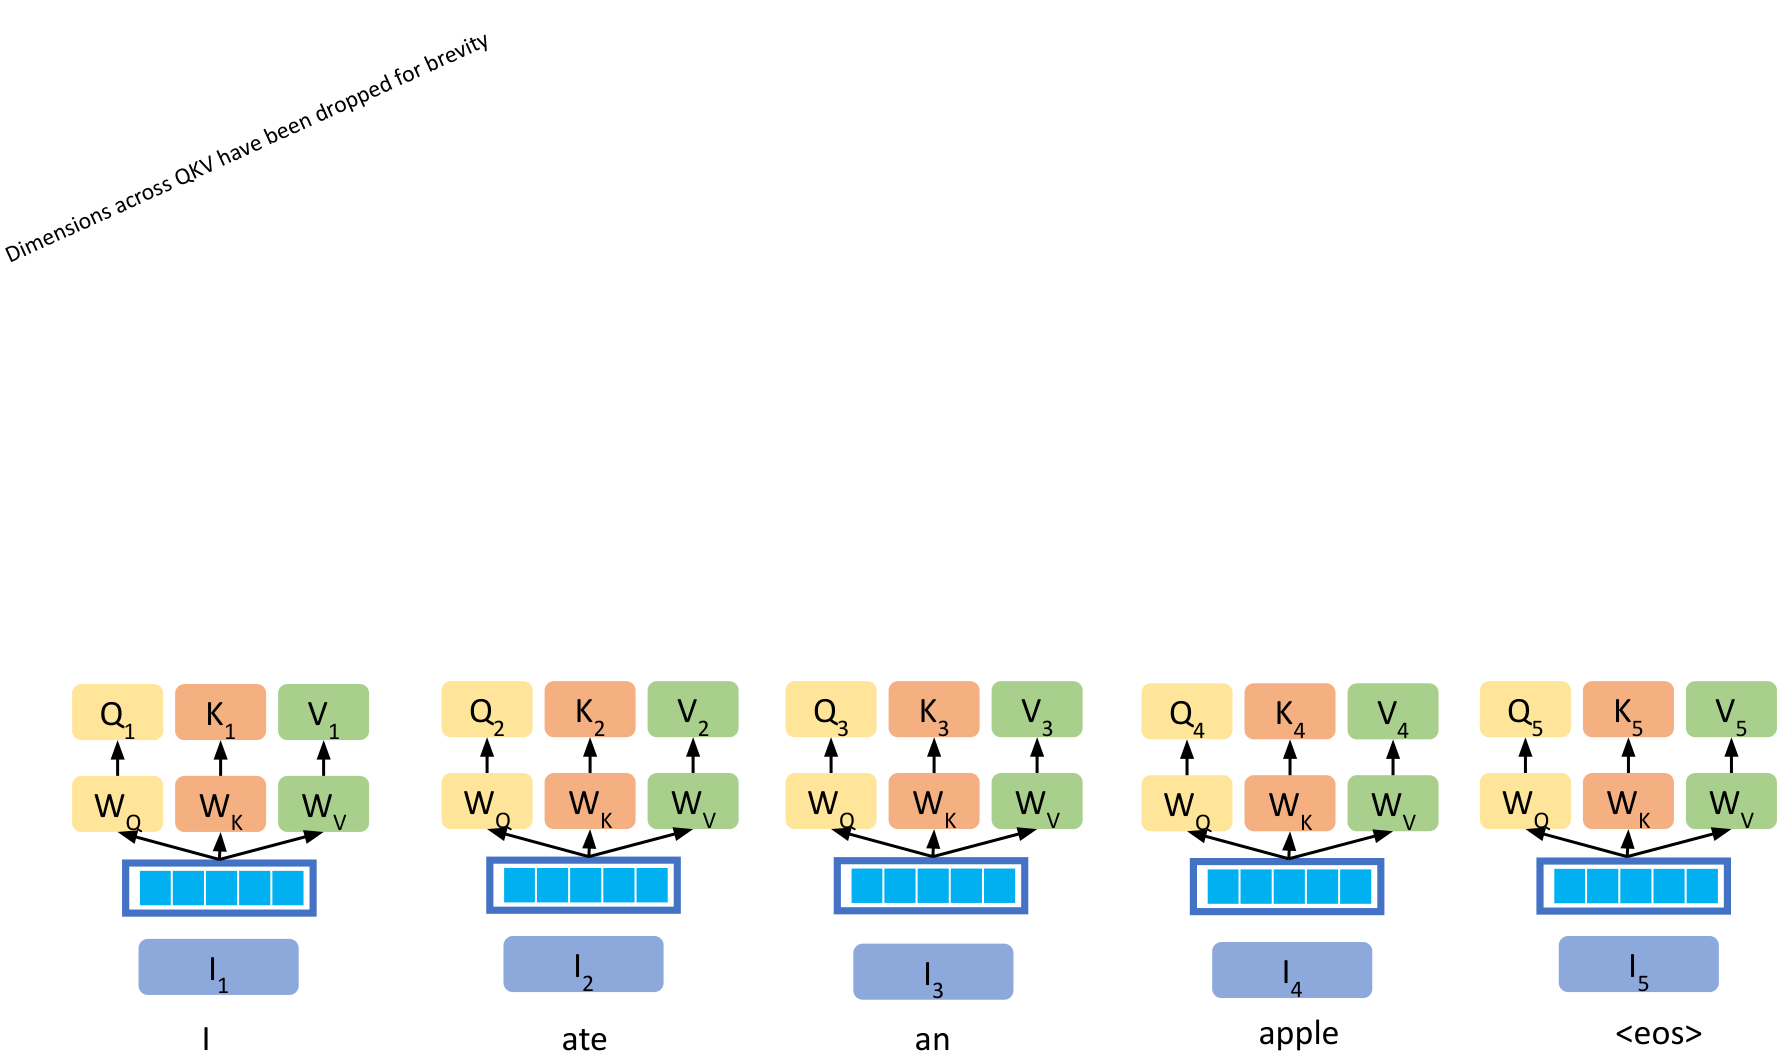
\includegraphics[width=0.7\paperwidth,height=0.66\paperheight,keepaspectratio]{images/attention-deep-dive/attention_qkv_projections_per_token.png}

  {\scriptsize Source: CMU 11-785 (Spring 2024), Lecture 19: Transformers and Newer Architectures, slide~47.}
\end{frame}

\begin{frame}{Attention}
  \centering
  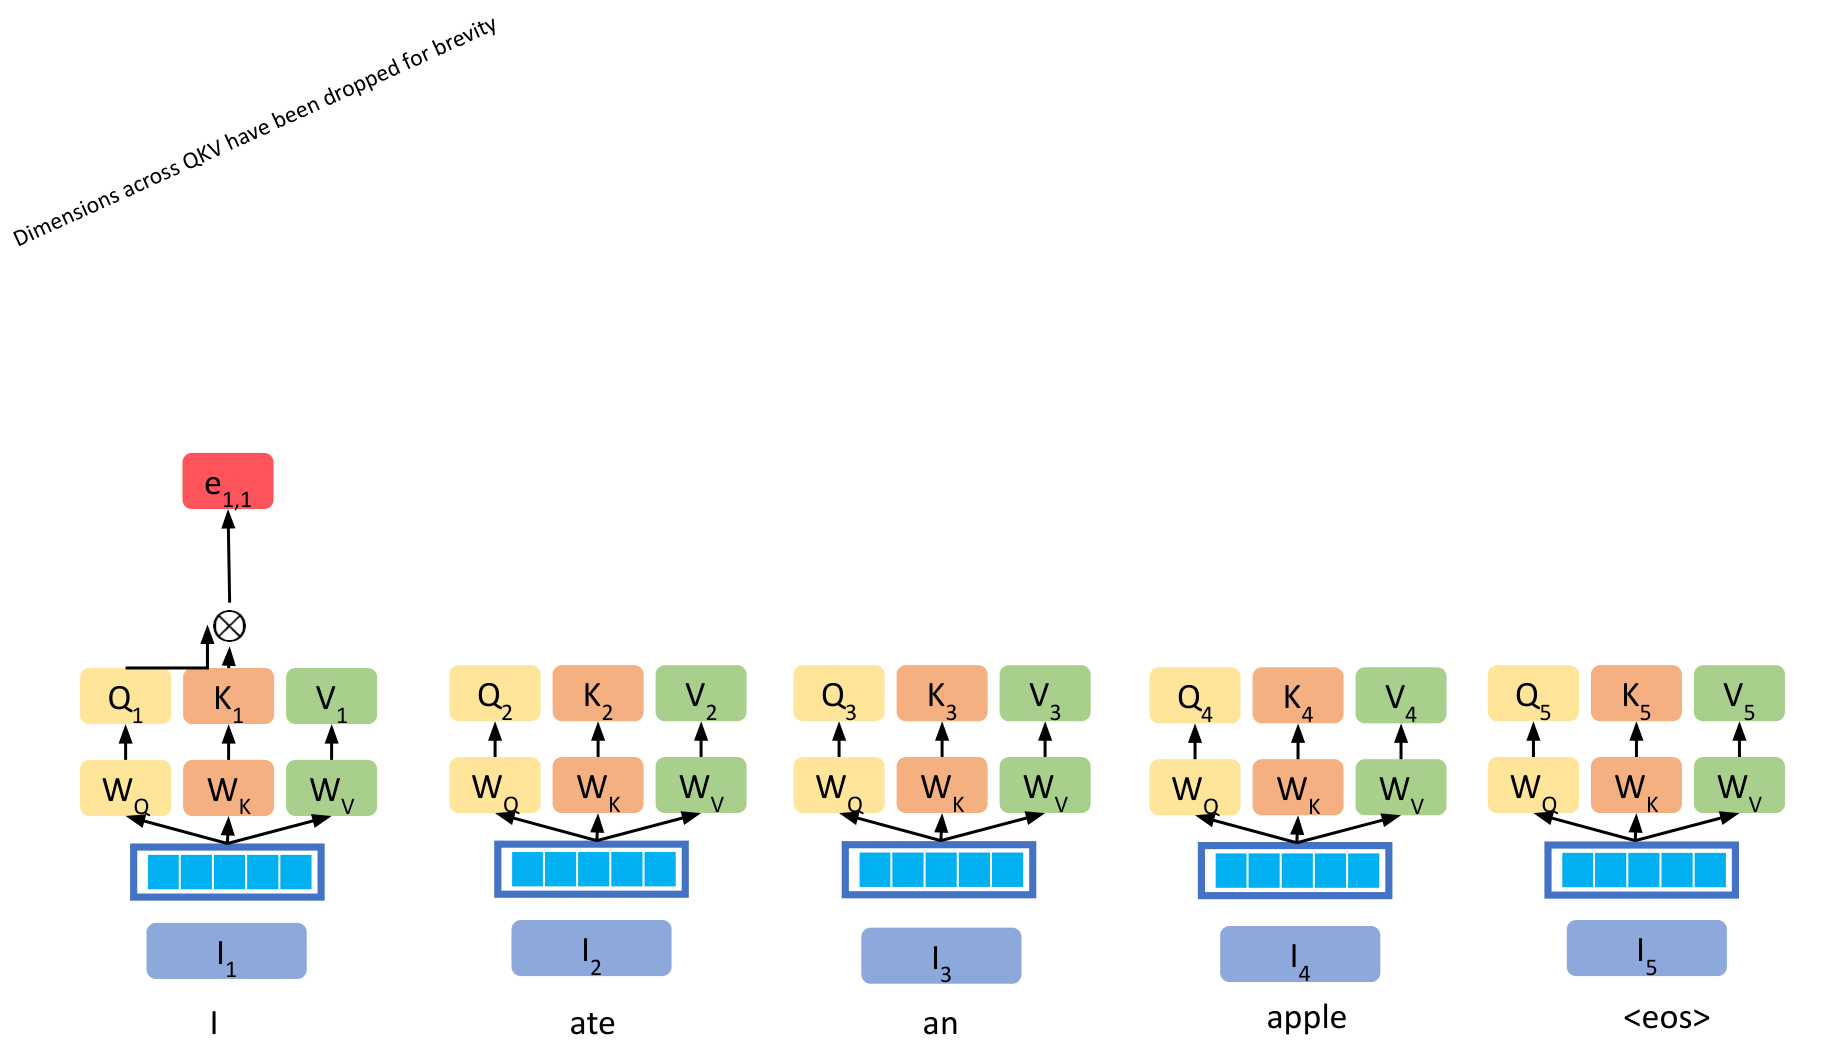
\includegraphics[width=0.7\paperwidth,height=0.66\paperheight,keepaspectratio]{images/attention-deep-dive/attention_score_e11_dotproduct.png}

  {\scriptsize Source: CMU 11-785 (Spring 2024), Lecture 19: Transformers and Newer Architectures, slide~48.}
\end{frame}

\begin{frame}{Attention}
  \centering
  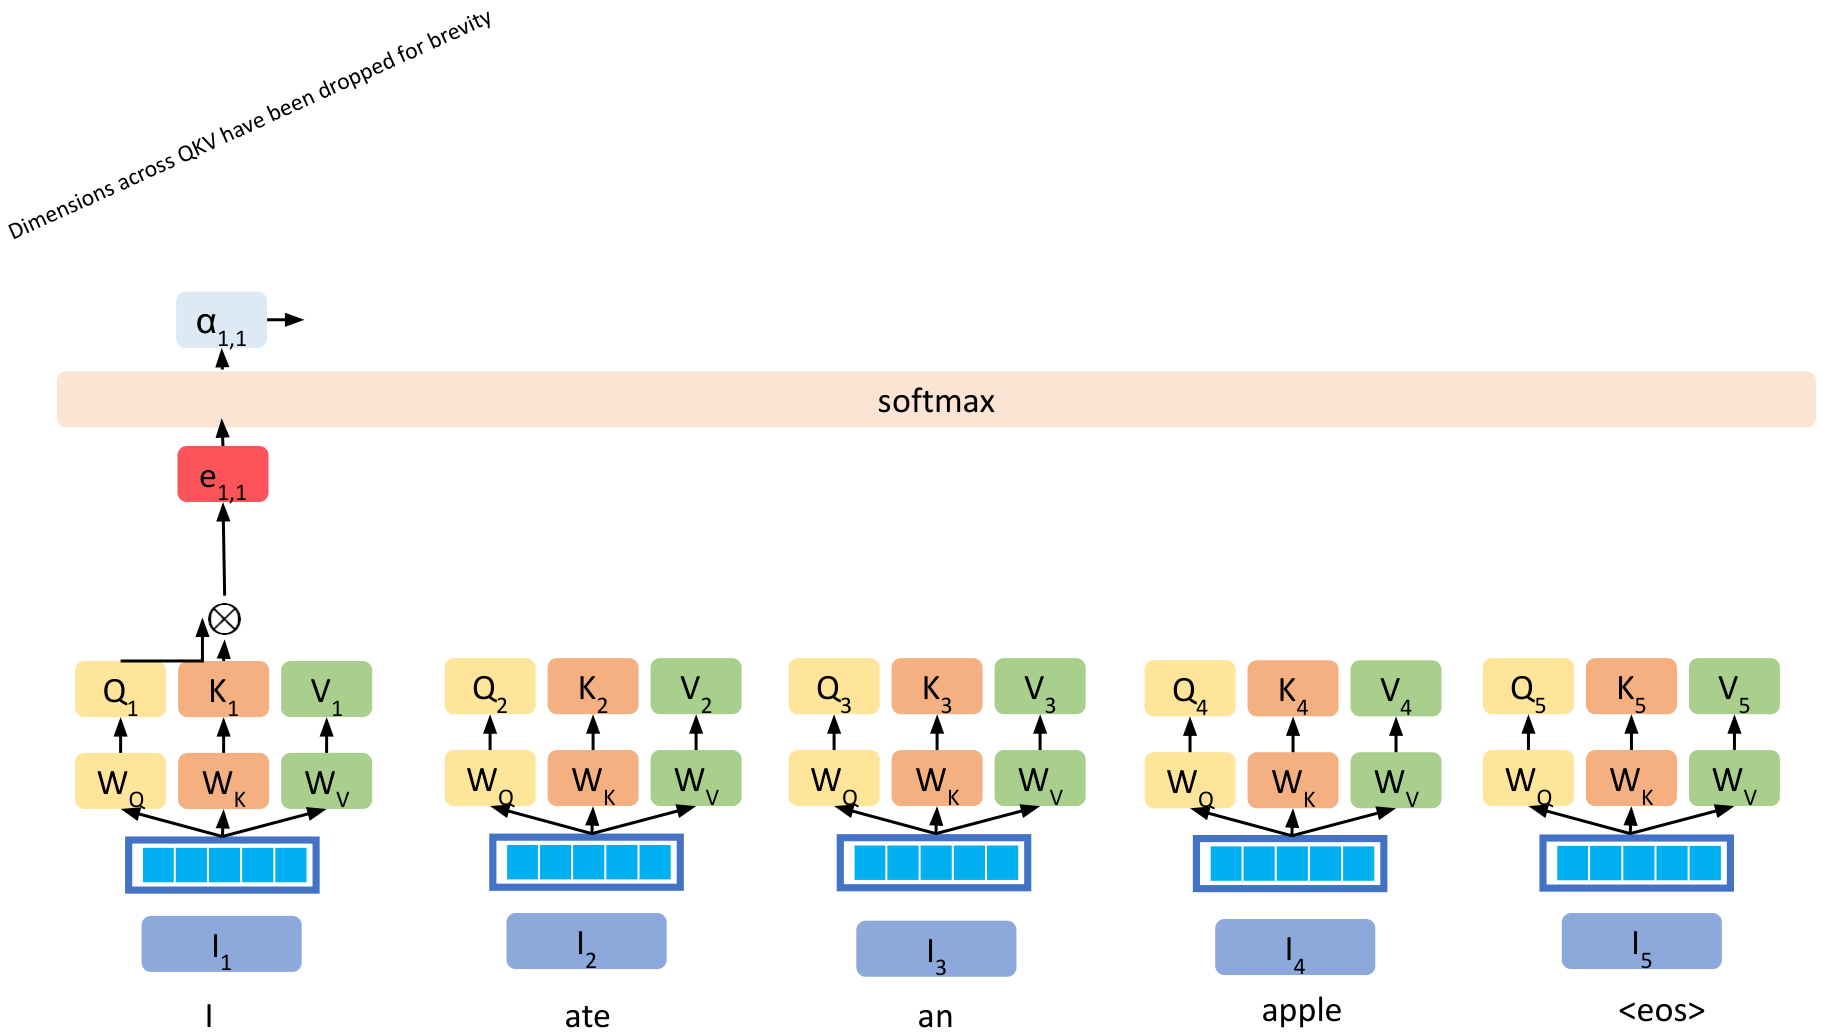
\includegraphics[width=0.7\paperwidth,height=0.66\paperheight,keepaspectratio]{images/attention-deep-dive/attention_softmax_alpha11.png}

  {\scriptsize Source: CMU 11-785 (Spring 2024), Lecture 19: Transformers and Newer Architectures, slide~49.}
\end{frame}

\begin{frame}{Attention}
  \centering
  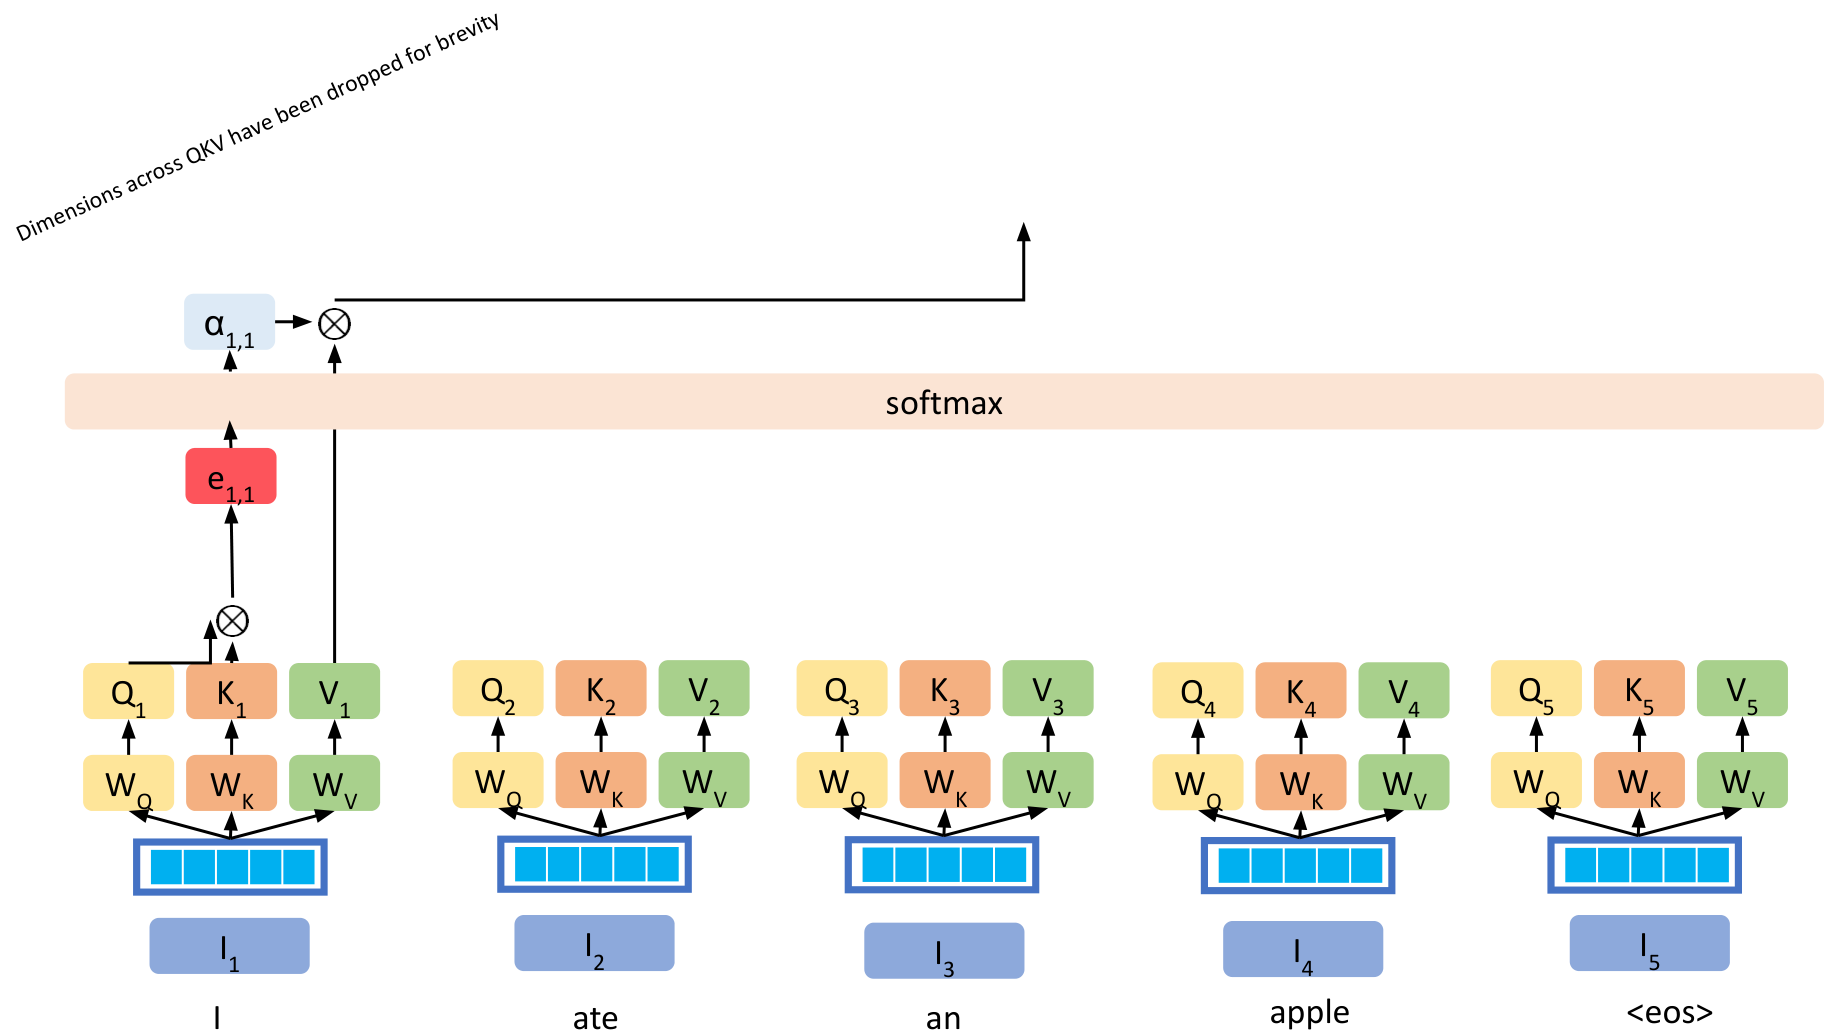
\includegraphics[width=0.7\paperwidth,height=0.66\paperheight,keepaspectratio]{images/attention-deep-dive/attention_weighted_value_first.png}

  {\scriptsize Source: CMU 11-785 (Spring 2024), Lecture 19: Transformers and Newer Architectures, slide~50.}
\end{frame}

\begin{frame}{Attention}
  \centering
  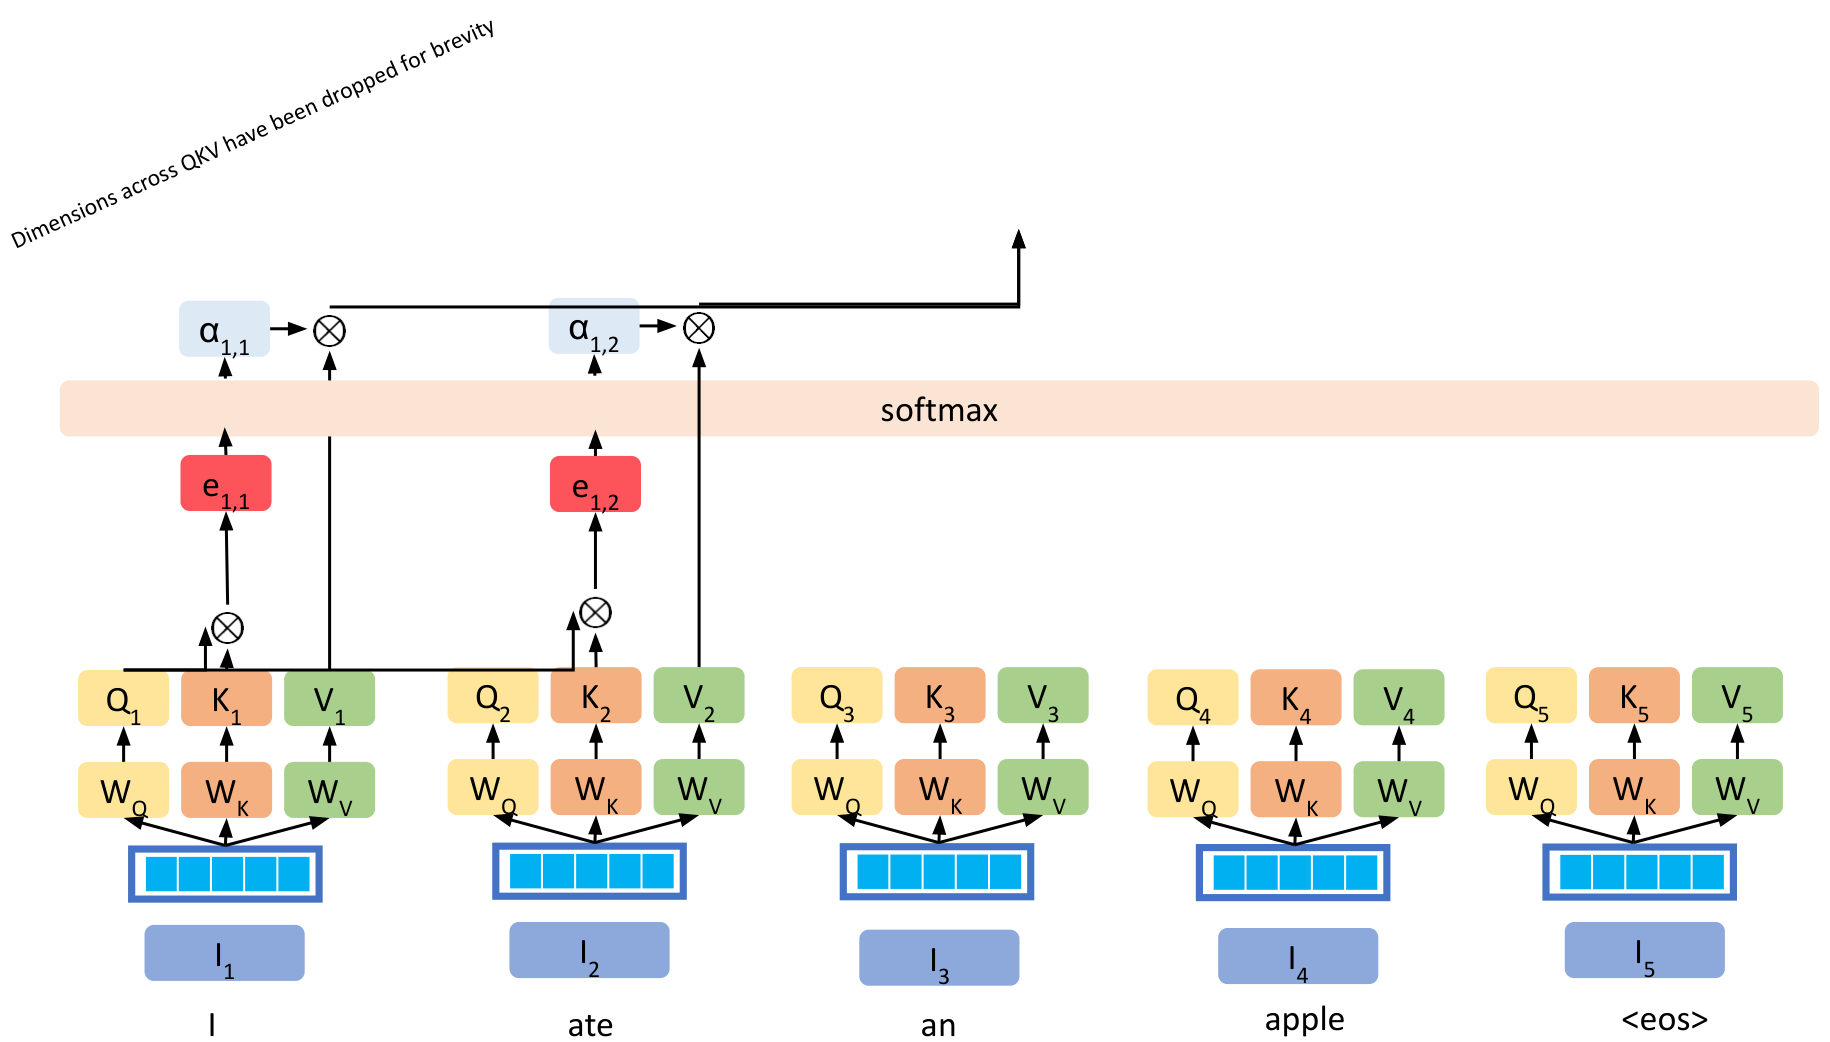
\includegraphics[width=0.7\paperwidth,height=0.66\paperheight,keepaspectratio]{images/attention-deep-dive/attention_two_scores_alpha12.png}

  {\scriptsize Source: CMU 11-785 (Spring 2024), Lecture 19: Transformers and Newer Architectures, slide~51.}
\end{frame}

\begin{frame}{Attention}
  \centering
  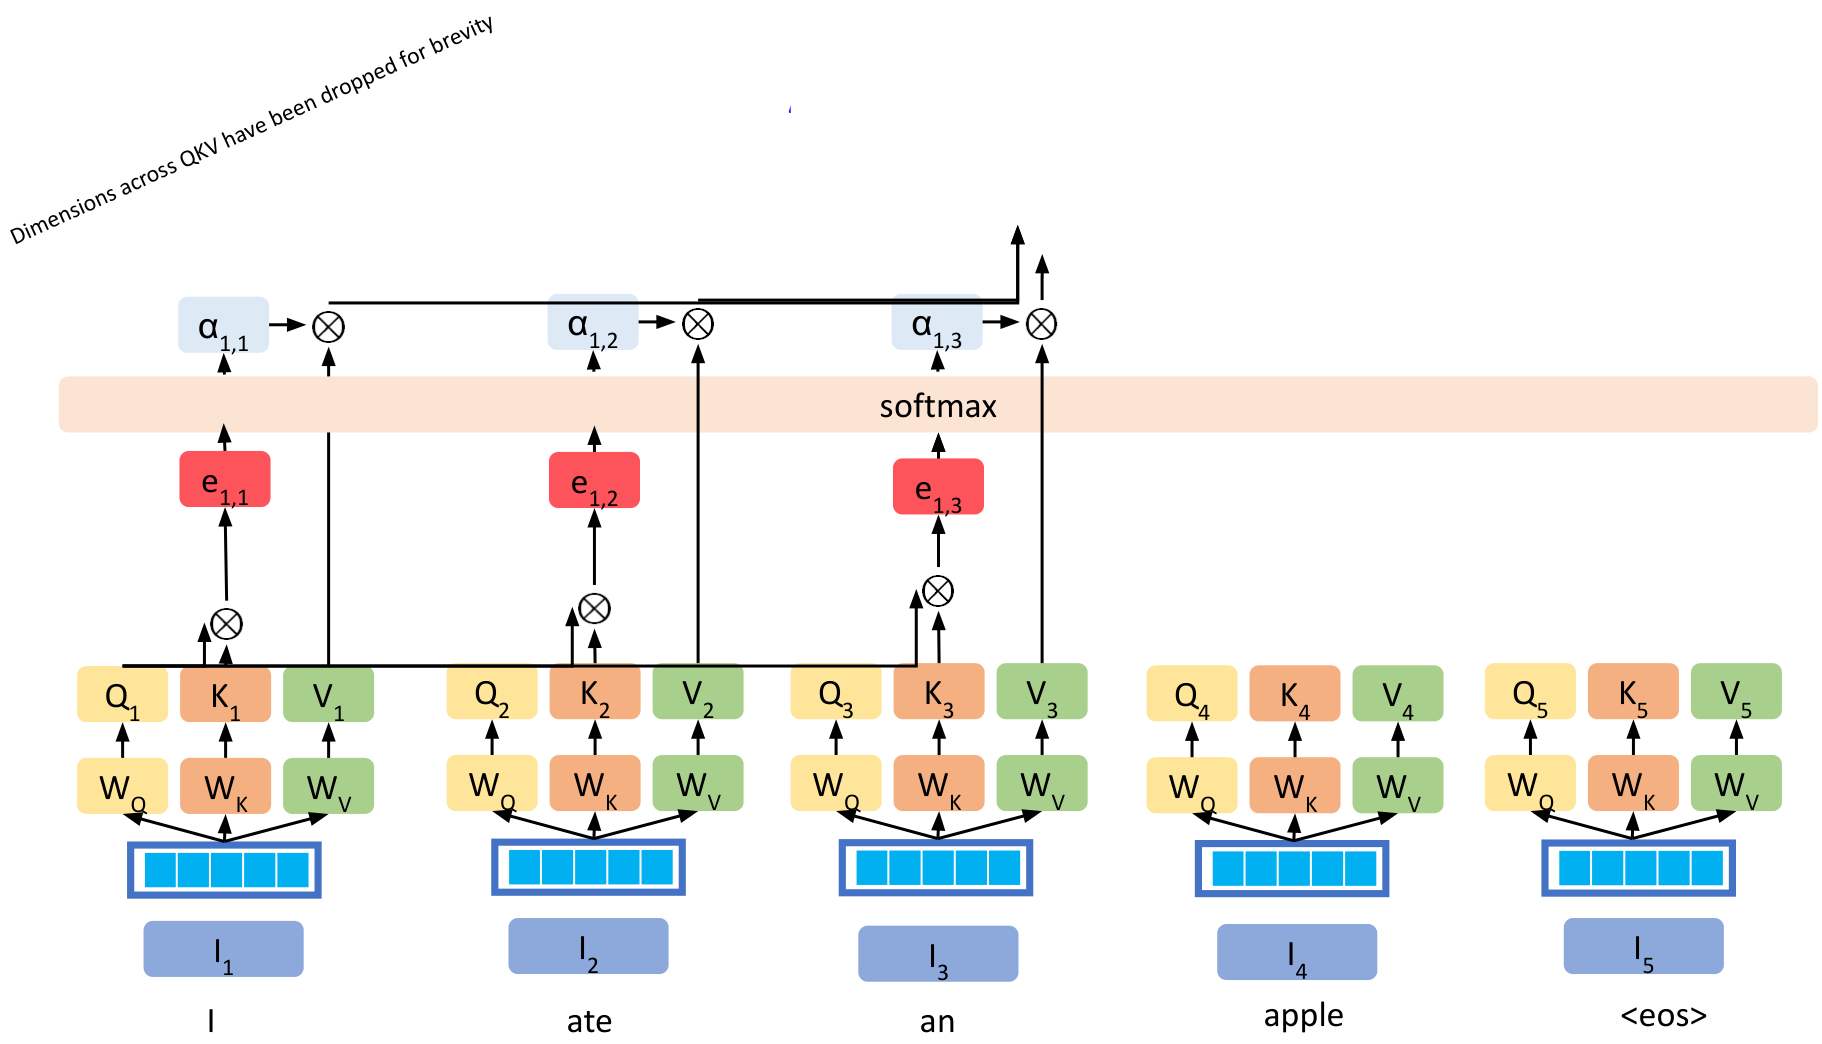
\includegraphics[width=0.7\paperwidth,height=0.66\paperheight,keepaspectratio]{images/attention-deep-dive/attention_three_scores_alpha13.png}

  {\scriptsize Source: CMU 11-785 (Spring 2024), Lecture 19: Transformers and Newer Architectures, slide~52.}
\end{frame}

\begin{frame}{Attention}
  \centering
  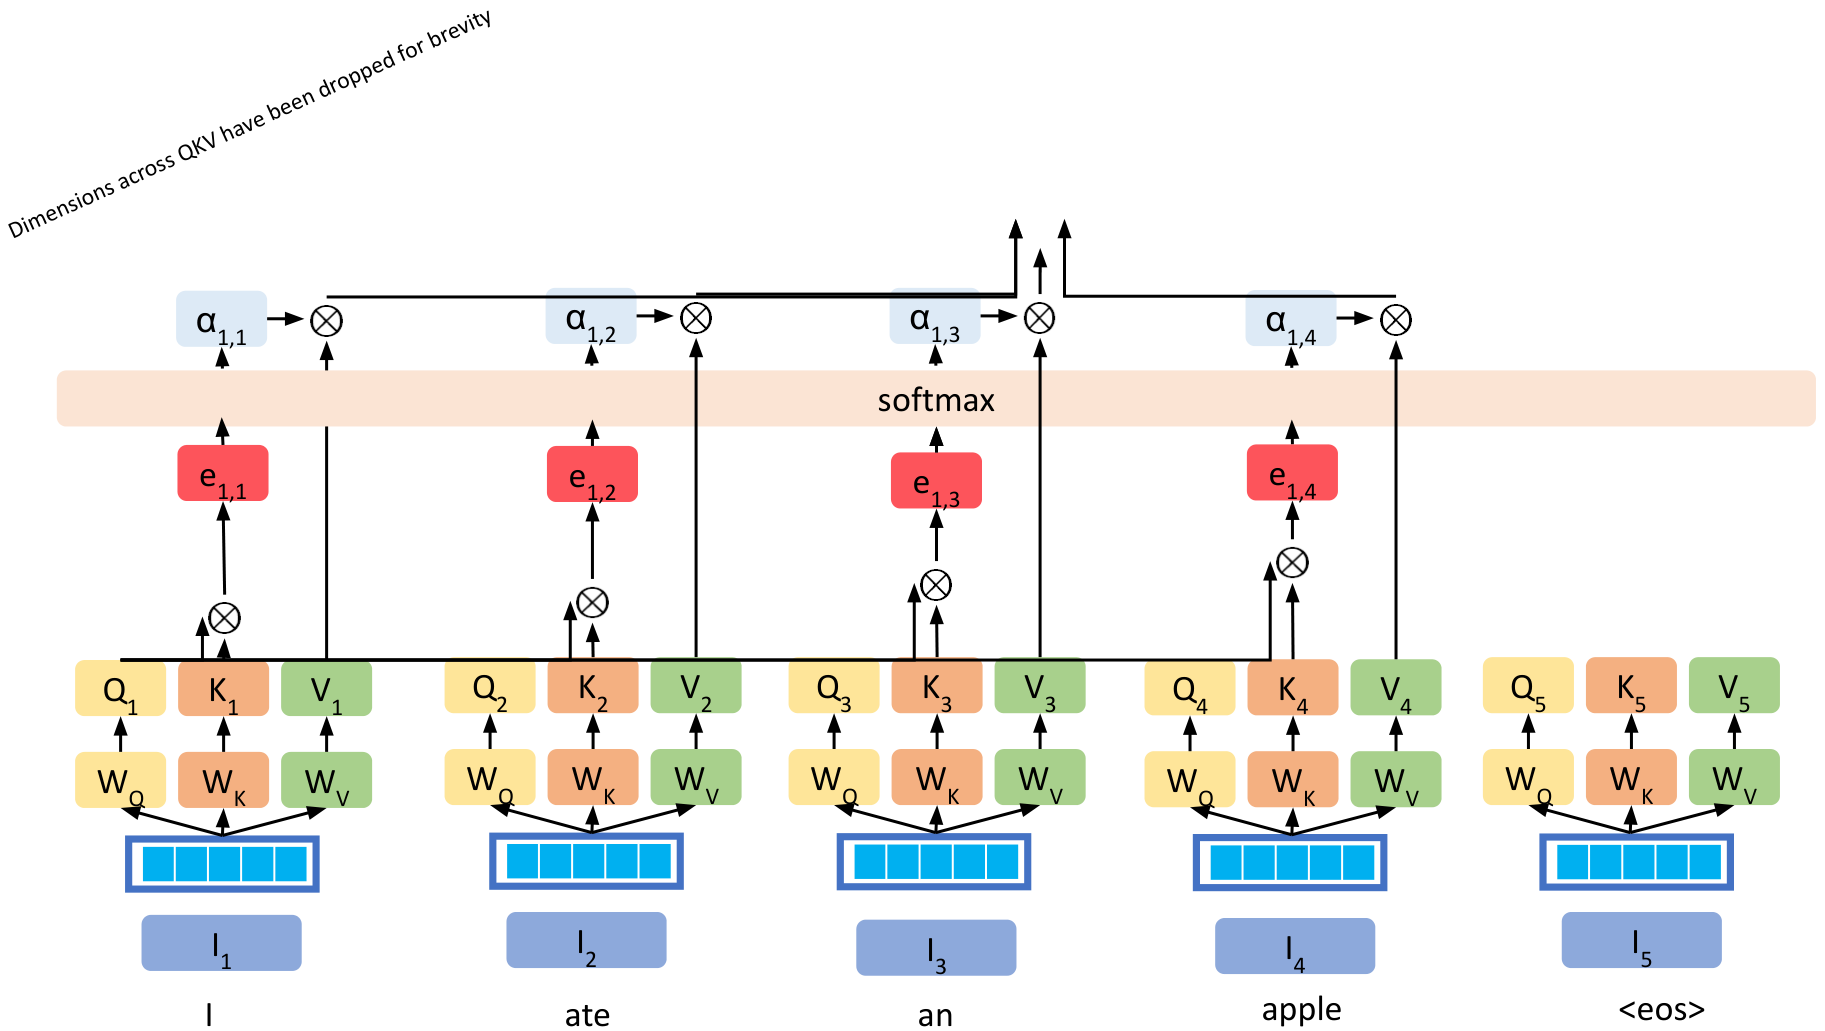
\includegraphics[width=0.7\paperwidth,height=0.66\paperheight,keepaspectratio]{images/attention-deep-dive/attention_four_scores_alpha14.png}

  {\scriptsize Source: CMU 11-785 (Spring 2024), Lecture 19: Transformers and Newer Architectures, slide~53.}
\end{frame}

\begin{frame}{Attention}
  \centering
  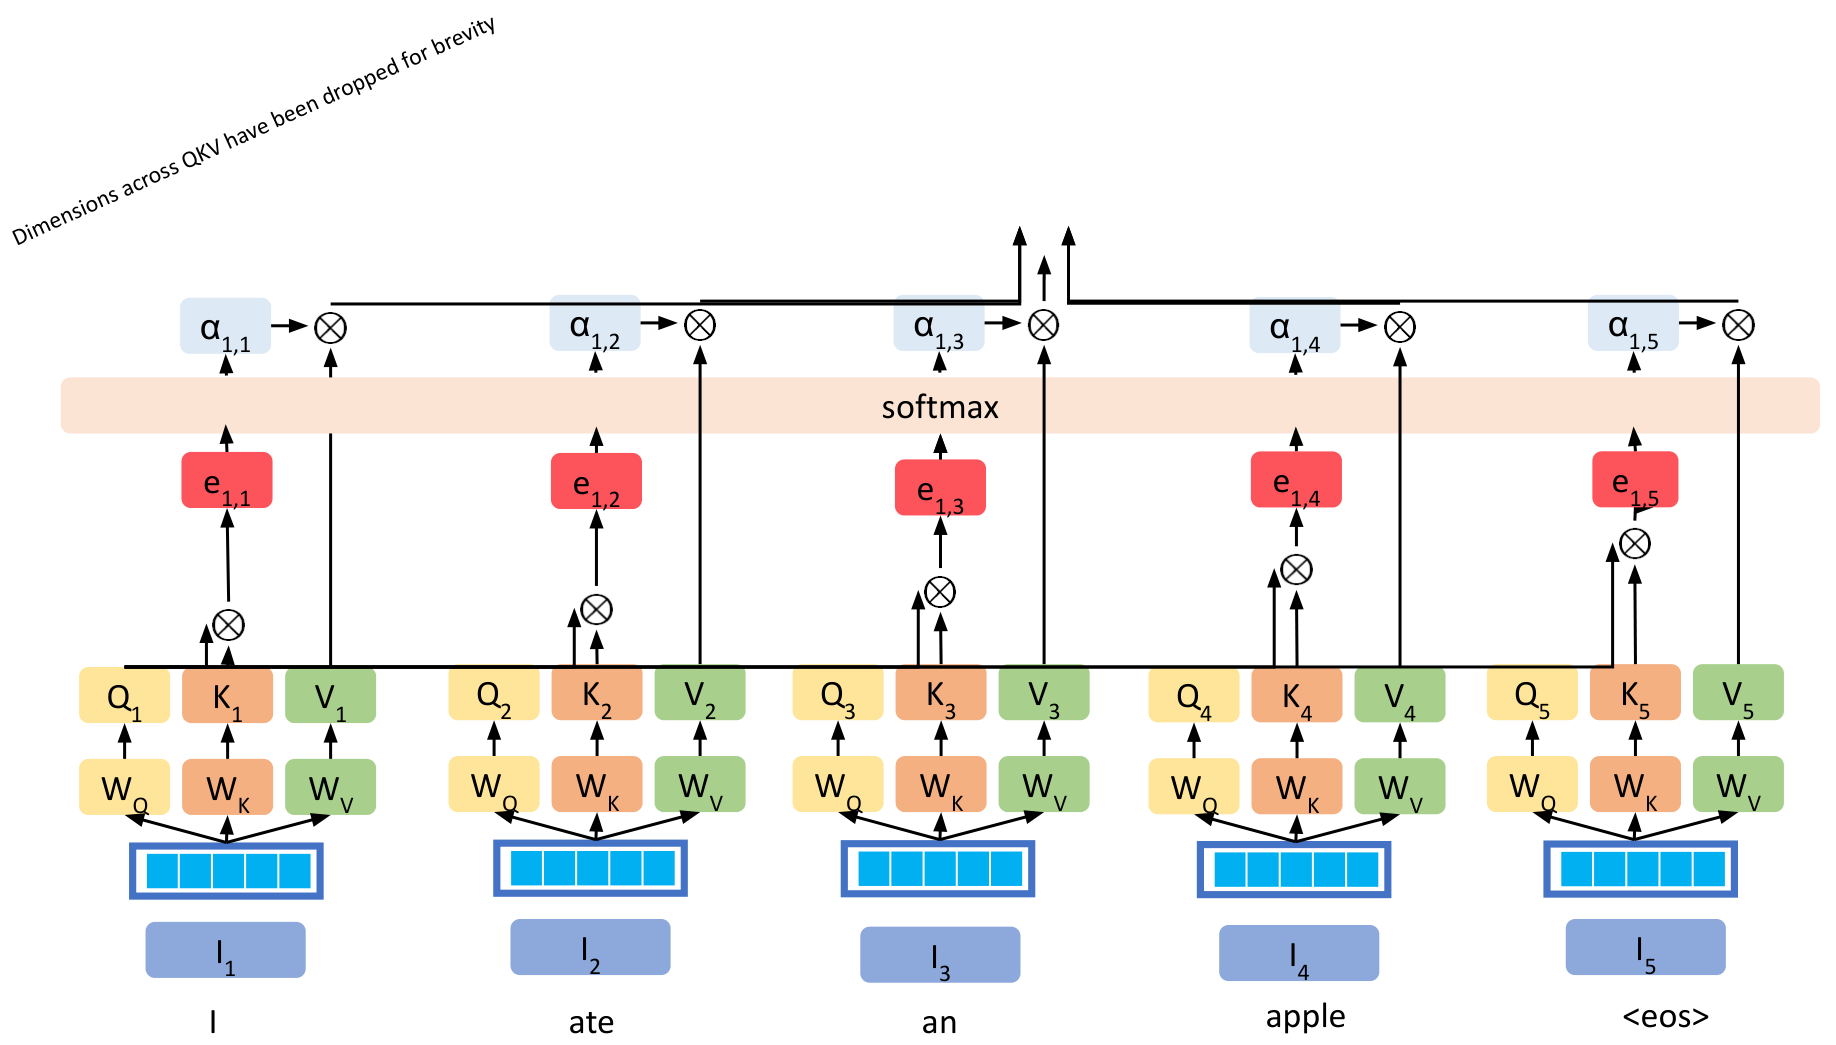
\includegraphics[width=0.7\paperwidth,height=0.66\paperheight,keepaspectratio]{images/attention-deep-dive/attention_five_scores_alpha15.png}

  {\scriptsize Source: CMU 11-785 (Spring 2024), Lecture 19: Transformers and Newer Architectures, slide~54.}
\end{frame}

\begin{frame}{Attention}
  \centering
  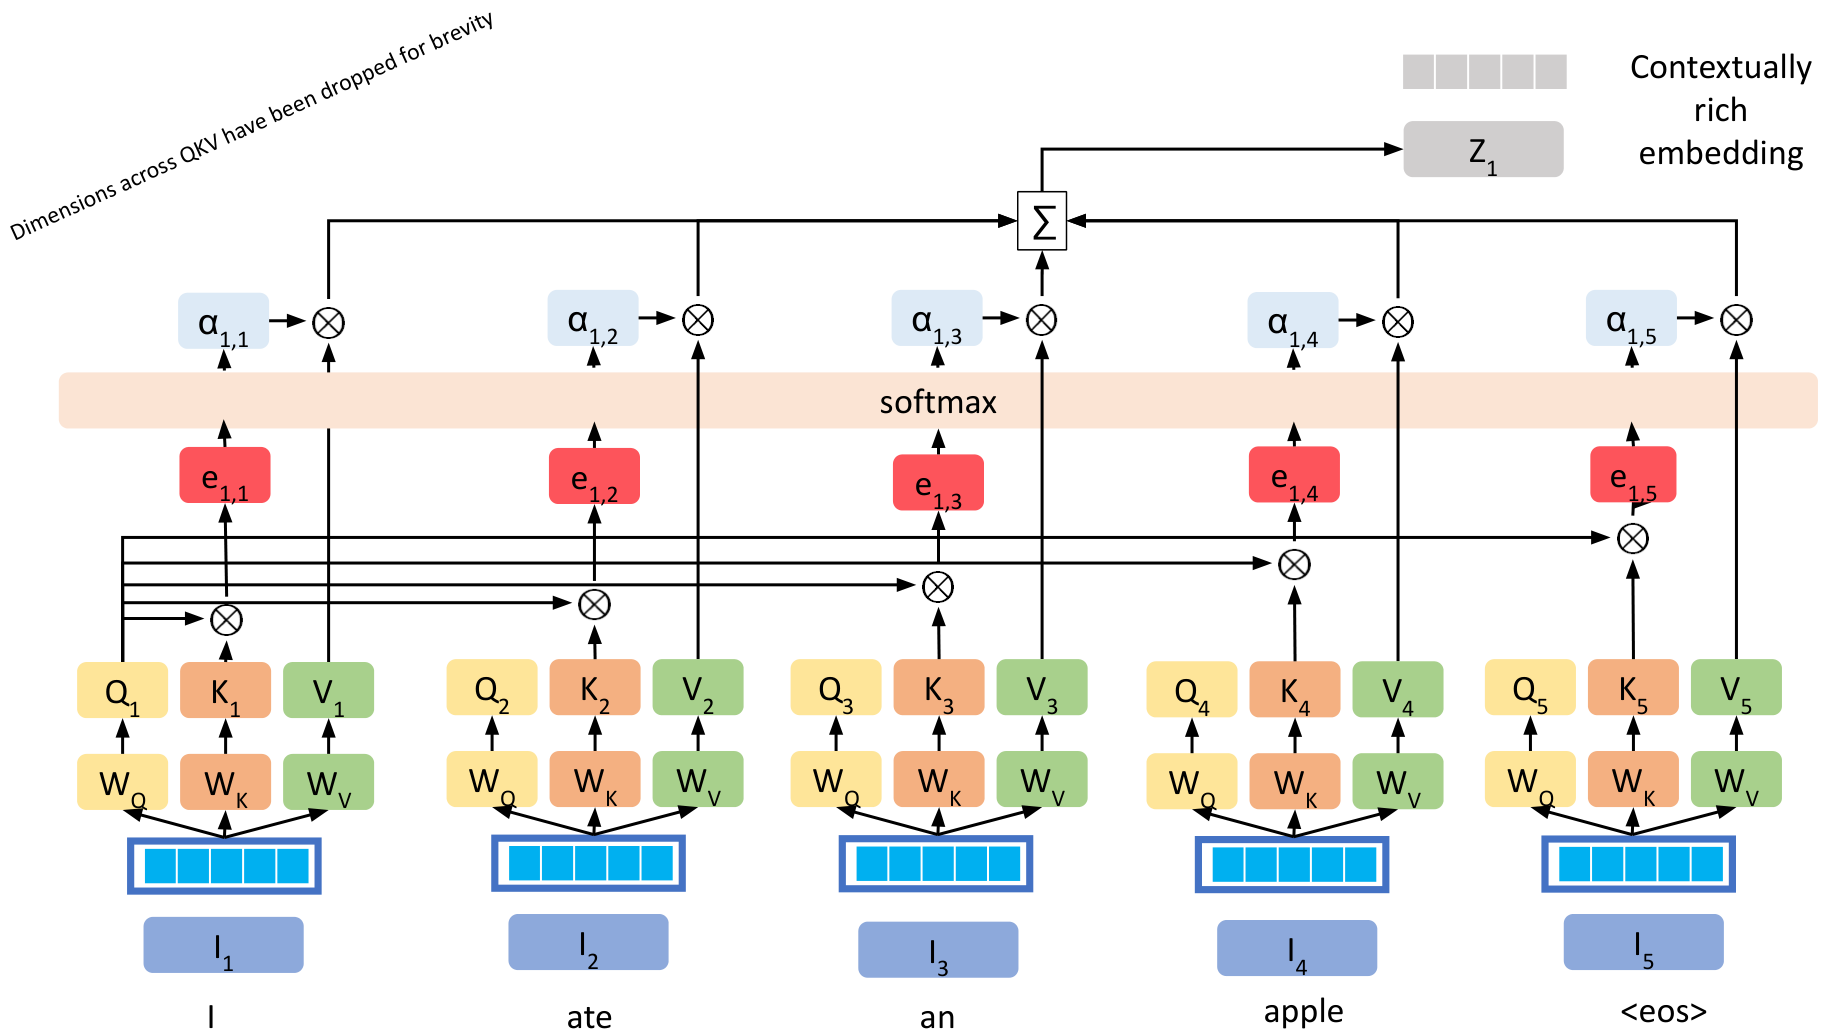
\includegraphics[width=0.7\paperwidth,height=0.66\paperheight,keepaspectratio]{images/attention-deep-dive/attention_weighted_sum_z1.png}

  {\scriptsize Source: CMU 11-785 (Spring 2024), Lecture 19: Transformers and Newer Architectures, slide~55.}
\end{frame}

\begin{frame}{Attention}
  \centering
  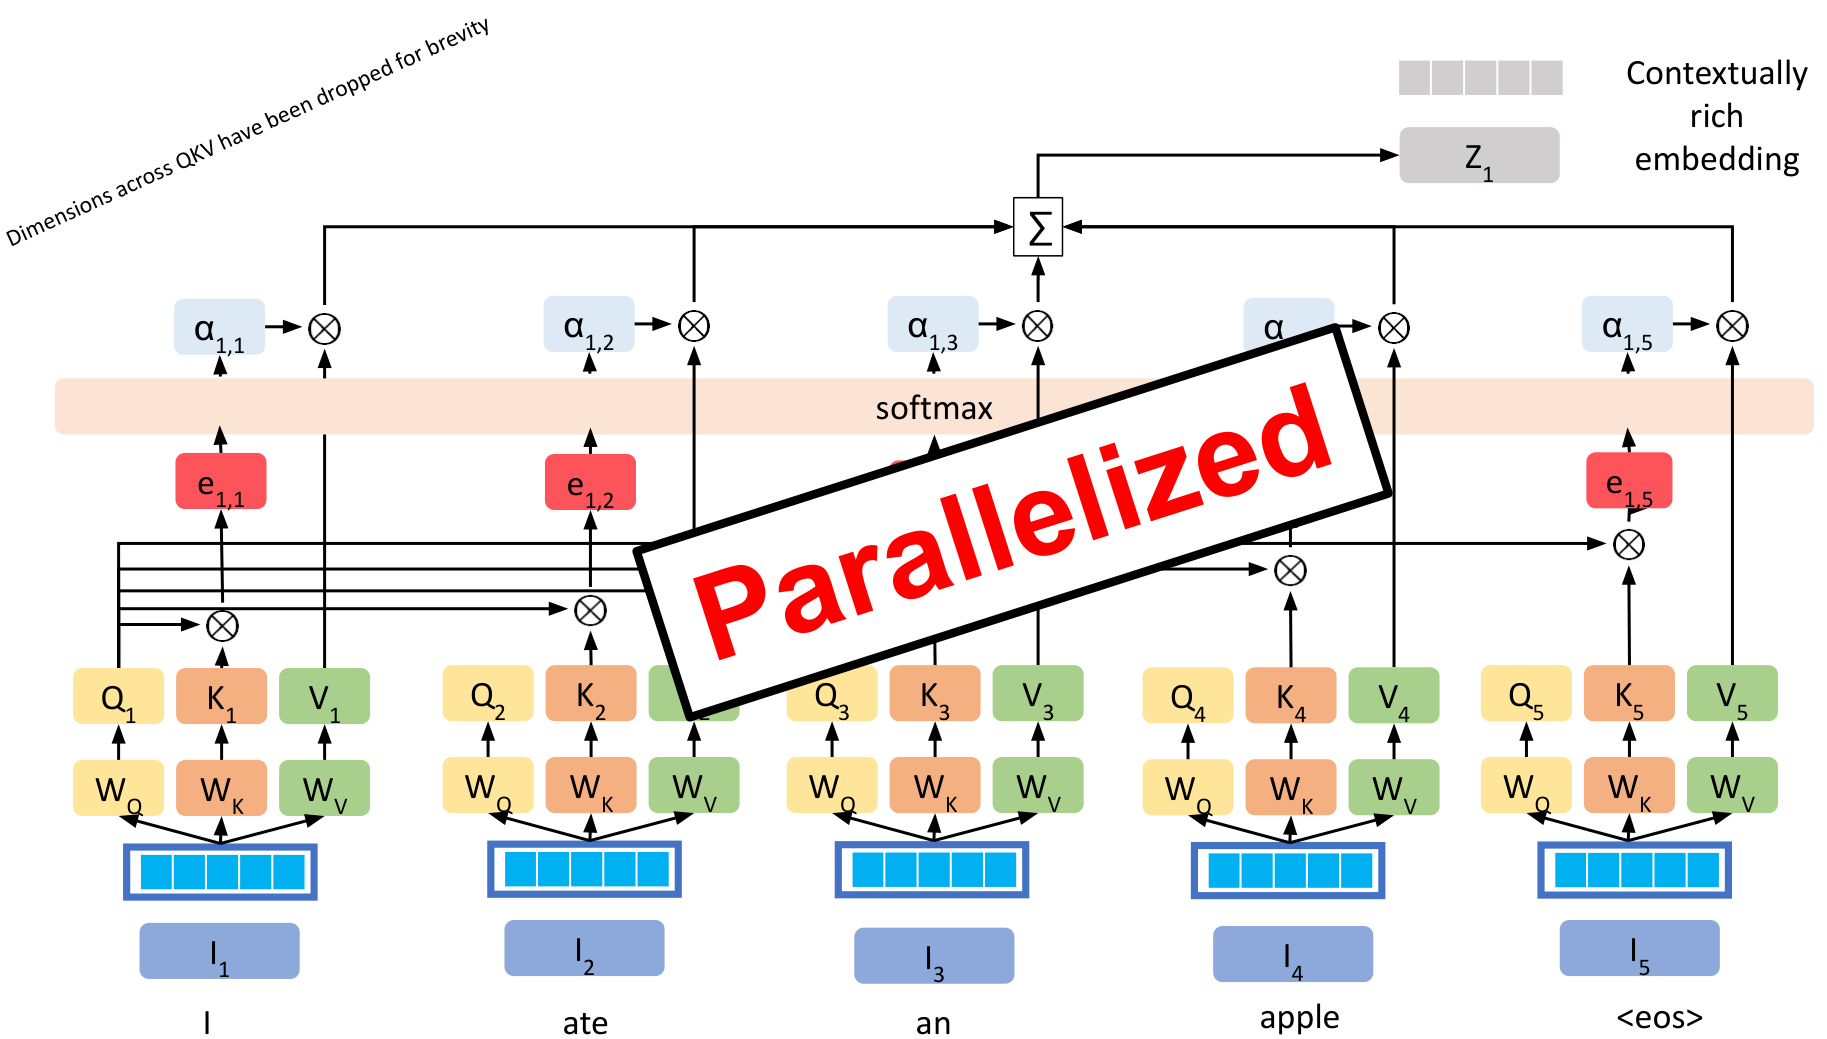
\includegraphics[width=0.7\paperwidth,height=0.66\paperheight,keepaspectratio]{images/attention-deep-dive/attention_self_attention_parallelized.png}

  {\scriptsize Source: CMU 11-785 (Spring 2024), Lecture 19: Transformers and Newer Architectures, slide~56.}
\end{frame}

\begin{frame}{Attention}
  \centering
  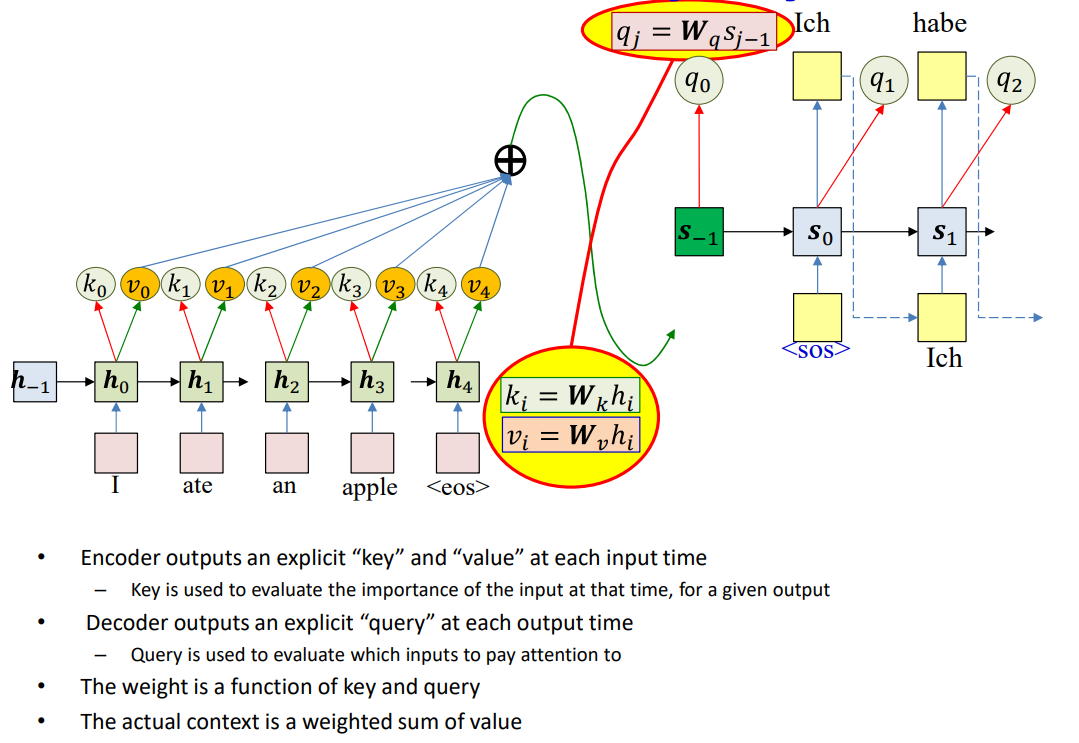
\includegraphics[width=0.7\paperwidth,height=0.66\paperheight,keepaspectratio]{images/attention-deep-dive/attention_decoder_key_value_query.png}

  {\scriptsize Source: CMU 11-785 (Spring 2024), Lecture 18: Sequence to Sequence Models \& Attention, slide~58.}
\end{frame}

\begin{frame}{Attention}
  \centering
  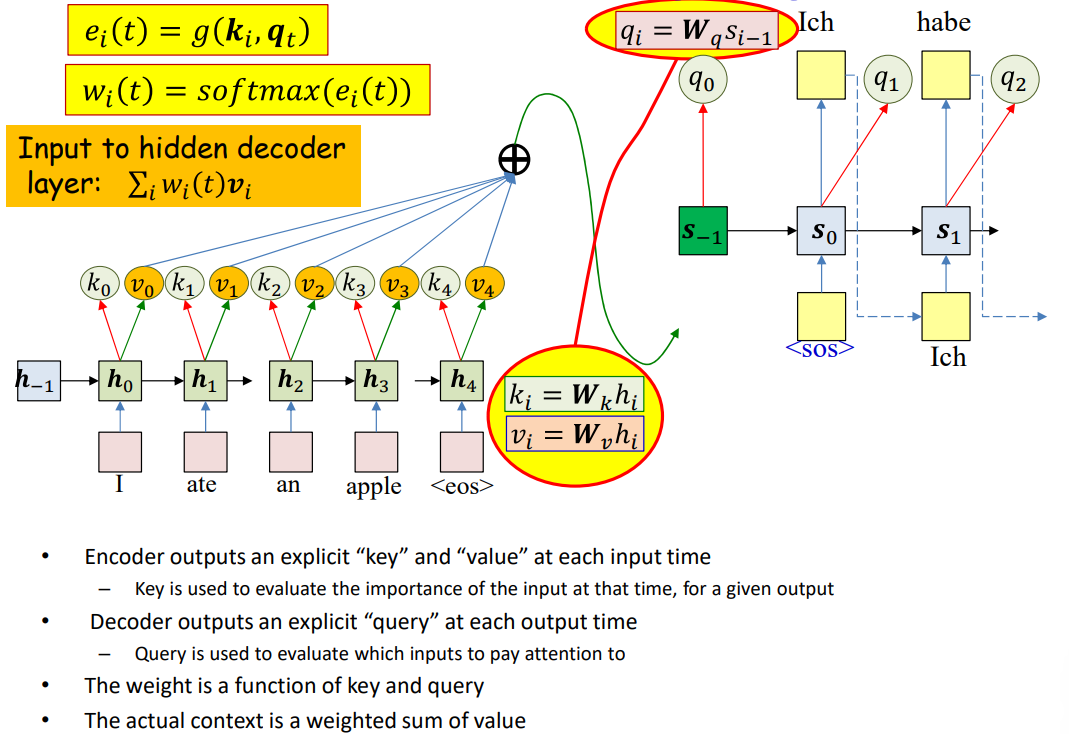
\includegraphics[width=0.7\paperwidth,height=0.66\paperheight,keepaspectratio]{images/attention-deep-dive/attention_decoder_context_formula.png}

  {\scriptsize Source: CMU 11-785 (Spring 2024), Lecture 18: Sequence to Sequence Models \& Attention, slide~59.}
\end{frame}

\begin{frame}{Attention}
  \centering
  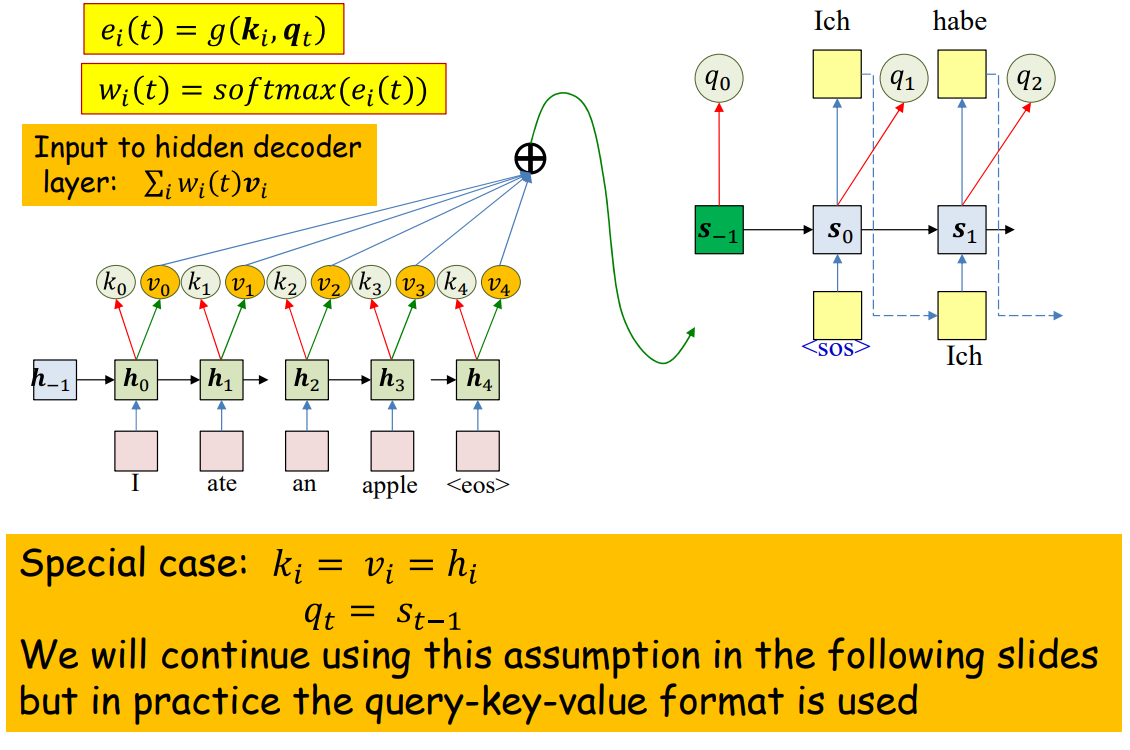
\includegraphics[width=0.7\paperwidth,height=0.66\paperheight,keepaspectratio]{images/attention-deep-dive/attention_special_case_kv_equals_h.png}

  {\scriptsize Source: CMU 11-785 (Spring 2024), Lecture 18: Sequence to Sequence Models \& Attention, slide~60.}
\end{frame}

\begin{frame}{Attention}
  \centering
  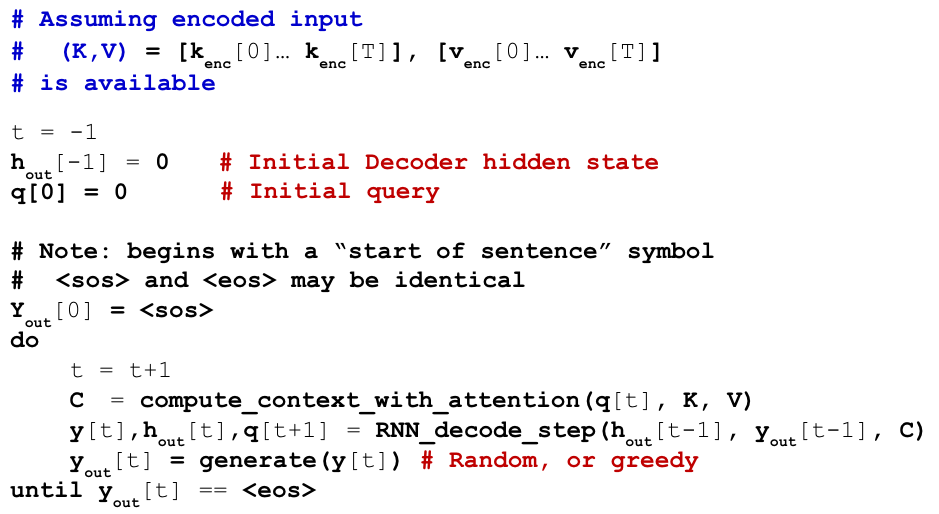
\includegraphics[width=0.7\paperwidth,height=0.66\paperheight,keepaspectratio]{images/attention-deep-dive/attention_decoder_pseudocode.png}

  {\scriptsize Source: CMU 11-785 (Spring 2024), Lecture 18: Sequence to Sequence Models \& Attention, slide~61.}
\end{frame}

\begin{frame}{Decoding -- Example: Translation}
\textbf{Example: English to French Translation}

\vspace{0.7em}

\begin{itemize}
  \item[] \textbf{Source Sentence (English)}\\
  \textit{The cat sat on the mat.}
  \vspace{0.3em}
  \item[] \textbf{Target Sentence (French)}\\
  \textit{Le chat s'est assis sur le tapis.}
\end{itemize}

\vspace{0.4em}

\begin{itemize}
  \item[$\blacktriangleright$] At each decoding step, the decoder generates a French word by:
    \begin{enumerate}
      \item Using the current decoder hidden state.
      \item Attending to relevant English words via attention weights.
      \item Computing a context vector as a weighted sum of encoder outputs.
    \end{enumerate}
  \item[$\blacktriangleright$] For example, when generating ``\textit{chat}'', the attention focuses on ``cat''.
  \item[$\blacktriangleright$] The process repeats for each word, dynamically shifting attention.
\end{itemize}

\end{frame}
